\section{Phương pháp nghiên cứu}\label{sec:intro}
\frame{\tableofcontents[currentsection]}
\subsection{Thay đổi, thử nghiệm và cải tiến mô hình có sẳn để tăng độ chính xác}
\begin{frame}{Thay đổi, thử nghiệm và cải tiến mô hình có sẳn để tăng độ chính xác}

\begin{itemize}
    \item Tiến hành cài đặt và thử nghiệm các công trình có độ chính xác cao trong những năm gần đây.
    \begin{itemize}
        \item Relation Aware Pedestrian Attribute Recognition with Graph Convolutional Networks [\ref{refer:1}]
        \item Improving Pedestrian Attribute Recognition With Weakly Supervised Multi Scale Attribute Specific Localization [\ref{refer:2}]
    \end{itemize}
    \item Từ các thử nghiệm trên tiến hành phân tích ưu và nhược điểm của công trình.
    \item Cải tiến mô hình bằng cách khắc phục những nhược điểm trên. Có thể tăng độ chính xác, giảm các trọng số học, giảm thời gian huấn luyện, ...
\end{itemize}
\end{frame}

\begin{frame}{Tổng quan về bài báo [\ref{refer:2}]}
\begin{itemize}
    \item Kiến trúc mạng
    % \begin{figure}[H]
    % \centering
    % 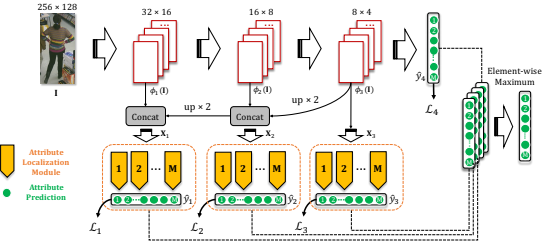
\includegraphics[width=12cm]{images/model_ALM.png}
    % \label{fig:model_ALM}
    % \end{figure}
\end{itemize}
\end{frame}

\begin{frame}{Tổng quan về bài báo [\ref{refer:2}]}
\begin{itemize}
    \item Kiến trúc mạng của ALM
    % \begin{figure}[H]
    % \centering
    % 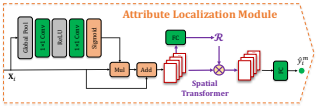
\includegraphics[width=8cm]{images/ALM.png}
    % \label{fig:ALM}
    % \end{figure}
    \item Ưu điểm: Kết hợp đặc trưng toàn cục và cục bộ, ALM đã tập trung tốt vào những vùng cần học, STN tự động làm giàu dữ liệu.
    \item Cải thiện: Channel Attention nên được sử dụng chung cho các channel để giảm các trọng số học.
\end{itemize}
\end{frame}

\subsection{Xây dựng mô hình mới để giải quyết bài toán}
\begin{frame}{Xây dựng mô hình mới để giải quyết bài toán}
\end{frame}
